\documentclass[preview]{standalone}
\usepackage{tikz}
\usepackage{fancyvrb}
\usepackage{xcolor}
\usepackage{soul}

\usetikzlibrary{positioning}
\usetikzlibrary{decorations.pathmorphing}
\usetikzlibrary{arrows.meta}

\usetikzlibrary{shadows}
\tikzset{
diagonal fill/.style 2 args={fill=#2, path picture={
\fill[#1, sharp corners] (path picture bounding box.south west) -|
                         (path picture bounding box.north east) -- cycle;}},
reversed diagonal fill/.style 2 args={fill=#2, path picture={
\fill[#1, sharp corners] (path picture bounding box.north west) |- 
                         (path picture bounding box.south east) -- cycle;}}
}

\begin{document}
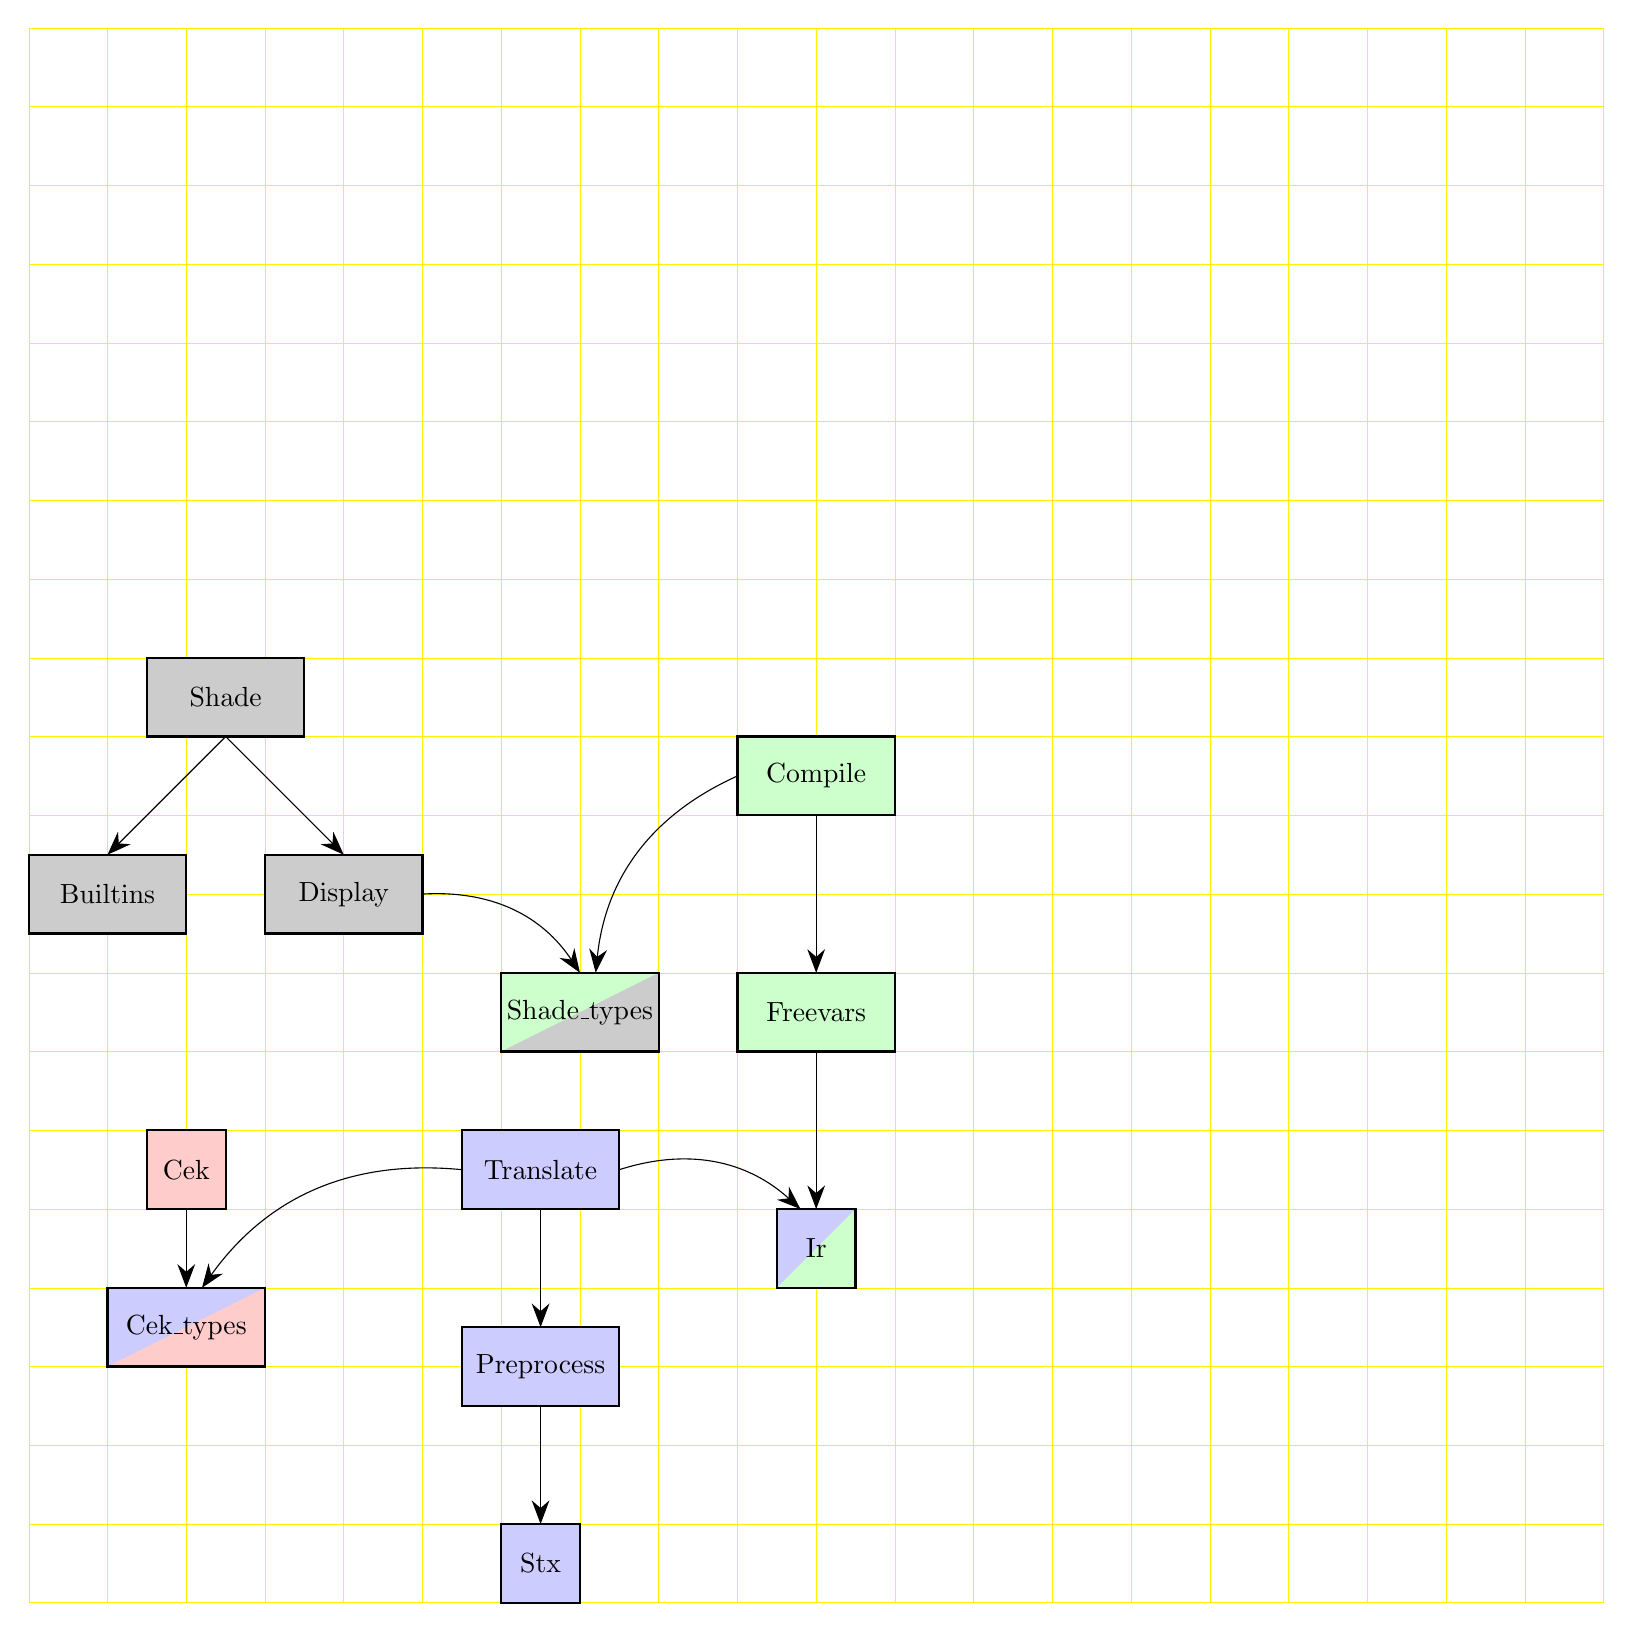
\begin{tikzpicture}
\draw[step=1cm,yellow,very thin] (0,0) grid (20,20);

% Coordinates
\coordinate (stx_top) at (6.5,1);
\coordinate (preprocess_bottom) at (6.5,2.5);
\coordinate (translate_bottom) at (6.5, 5);
\coordinate (preprocess_top) at (6.5,3.5);
\coordinate (freevars_top) at (10,8);
\coordinate (compile_bottom) at (10,10);
\coordinate (cek_bottom) at (2,5);
\coordinate (cek_types_top) at (2, 4);
\coordinate (cek_types_top2) at (2.2, 4);
\coordinate (ir_top) at (10, 5);
\coordinate (ir_top2) at (9.8, 5);
\coordinate (freevars_bottom) at (10, 7);
\coordinate (builtins_top) at (1,9.5);
\coordinate (display_top) at (4,9.5);
\coordinate (shade_types_top) at (7,8);
\coordinate (shade_types_top2) at (7.2,8);
\coordinate (shade_bottom) at (2.5, 11);
\coordinate (display_right) at (5,9);
\coordinate (compile_left) at (9,10);
\coordinate (compile_left) at (9,10.5);
\coordinate (translate_right) at (7.5,5.5);
\coordinate (ir_left) at (9.5,4.5);
\coordinate (translate_left) at (5.5,5.5);

% Boxes
\draw[black,thick,fill=blue!20] (6,0) rectangle (7,1) node[pos=.5] {Stx};
\draw[black,thick,fill=blue!20] (5.5,2.5) rectangle (7.5,3.5) node[pos=.5] {Preprocess};
\draw[black,thick,fill=blue!20] (5.5,5) rectangle (7.5,6) node[pos=.5] {Translate};

\draw[black,thick,diagonal fill={red!20}{blue!20}] (1,3) rectangle (3,4) node[pos=.5] {Cek\_types};
\draw[black,thick,fill=red!20] (1.5,5) rectangle (2.5,6) node[pos=.5] {Cek};

\draw[black,thick, diagonal fill={green!20}{blue!20}] (9.5,4) rectangle (10.5,5) node[pos=.5] {Ir};
\draw[black,thick, fill=green!20] (9,7) rectangle (11,8) node[pos=.5] {Freevars};
\draw[black,thick, fill=green!20] (9,10) rectangle (11,11) node[pos=.5] {Compile};

\draw[black,thick, fill=black!20] (0,8.5) rectangle (2,9.5) node[pos=.5] {Builtins};
\draw[black,thick, fill=black!20] (3,8.5) rectangle (5,9.5) node[pos=.5] {Display};
\draw[black,thick, diagonal fill={black!20}{green!20}] (6,7) rectangle (8,8) node[pos=.5] {Shade\_types};
\draw[black,thick, fill=black!20] (1.5,11) rectangle (3.5,12) node[pos=.5] {Shade};

% Arrows

\draw[-{Stealth[length=3mm]}] (preprocess_bottom) -- (stx_top);
\draw[-{Stealth[length=3mm]}] (translate_bottom) -- (preprocess_top);
\draw[-{Stealth[length=3mm]}] (compile_bottom) -- (freevars_top);
\draw[-{Stealth[length=3mm]}] (freevars_bottom) -- (ir_top);
\draw[-{Stealth[length=3mm]}] (cek_bottom) -- (cek_types_top);
\draw[-{Stealth[length=3mm]}] (shade_bottom) -- (builtins_top);
\draw[-{Stealth[length=3mm]}] (shade_bottom) -- (display_top);
\draw[-{Stealth[length=3mm]}] (display_right) to [bend left] (shade_types_top);
\draw[-{Stealth[length=3mm]}] (compile_left) to [bend right] (shade_types_top2);
\draw[-{Stealth[length=3mm]}] (translate_right) to [bend left] (ir_top2);
\draw[-{Stealth[length=3mm]}] (translate_left) to [bend right] (cek_types_top2);

\end{tikzpicture}

\end{document}
